\section{Theory and Framework}
\subsection{Framework Diagram and Full Covariance Derivation}
The accompanying NumPy implementation, \path{scripts/mira.py}, accepts a frozen estimator callable, physical anchor dictionaries, declared support and scale provenance, perturbation settings, and optional retrospective targets. It implements paired predictions, the all-anchor-energy influence statistic, and separate error evaluation. Model freezing and clustered aggregation remain caller responsibilities. Tests cover acquired-only target-mutation invariance, inconsistent shared-anchor rejection, energy closure, and a linear coefficient reference including perturbation-sign reversal. Reproduction instructions are in \path{REPRODUCIBILITY.md}.
\begin{figure*}[t]
\centering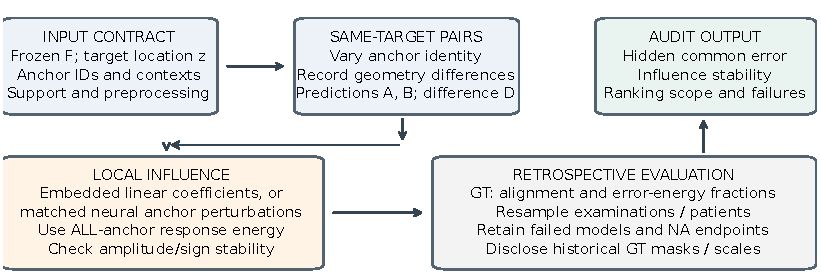
\includegraphics[width=.98\textwidth]{p17_framework.pdf}
\caption{The reusable Measurement-Influence Reliability Audit. The estimator is frozen. Physical anchor identities, support, preprocessing and source of each quantity are part of the input contract. Targets enter retrospective error evaluation; historical GT-mask and full-examination-scale exceptions are disclosed rather than relabeled as deployment inputs. This is a framework diagram, not a proposed reconstruction architecture.}
\label{fig:p17-framework}
\end{figure*}

Condition on fixed nominal inputs and a fixed target $y$. Write $e_a=b_a+J_a\xi_a$ and $e_b=b_b+J_b\xi_b$, where the perturbations have zero mean and finite second moments. Let $\Sigma_a=\mathbb E\xi_a\xi_a^\top$, $\Sigma_b=\mathbb E\xi_b\xi_b^\top$, and $C=\mathbb E\xi_a\xi_b^\top$, with the joint block covariance positive semidefinite. Then
\begin{align}
\mathbb E\langle e_a,e_b\rangle
 &=\langle b_a,b_b\rangle+\operatorname{tr}(J_a C J_b^\top),\\
\tau=\mathbb E T
 &=\tfrac12\{\|b_a\|^2+\|b_b\|^2+\operatorname{tr}(J_a\Sigma_aJ_a^\top)\nonumber\\
 &\hspace{28mm}+\operatorname{tr}(J_b\Sigma_bJ_b^\top)\}.
\end{align}
Changing $C$ from zero to a valid cross-covariance, with biases, Jacobians and marginals fixed, changes the first quantity by $\kappa=\operatorname{tr}(J_a C J_b^\top)$ and leaves $\tau$ unchanged. Therefore
\begin{align}
\Delta\mathbb E\|e_a-e_b\|^2&=-2\kappa,\\
\Delta\mathbb E\|(e_a-e_b)/2\|^2&=-\kappa/2,\\
\Delta\mathbb E\|(e_a+e_b)/2\|^2&=+\kappa/2.
\end{align}
For $\tau>0$, the ratio $\mathbb E\|(e_a-e_b)/2\|^2/\tau$ decreases by $\kappa/(2\tau)$ when $\kappa>0$. This ratio is not the expected samplewise fraction, and positive $\kappa$ does not establish a monotone change in each realized error cosine or each examination's rank.

\paragraph{Physical-anchor interpretation.}
If distinct physical anchors have independent perturbations and shared anchors reuse the same perturbation, $C$ has nonzero blocks only for shared identities. Thus $\kappa=\sum_{j\in c_a\cap c_b}\operatorname{tr}(J_{aj}\Sigma_jJ_{bj}^\top)$. Aligned sensitivities make these terms positive; orthogonal sensitivities can make sharing irrelevant, and opposing sensitivities can make it increase disagreement. Shared anchor count alone cannot determine the sign or magnitude. If the two contexts are perturbed by independent noise even on an identical anchor, this covariance mechanism is absent despite identical nominal anatomy. Common deterministic bias remains possible in either setting.

\paragraph{Finite responses.}
For $r_{cjs}=F_c(x+\epsilon\xi_{js})-F_c(x)$, local differentiability gives $r_{cjs}=\epsilon J_{cj}\xi_{js}+R_{cjs}$. Under the linear model and matched fields,
\begin{equation}
\mathbb E\left[\frac{1}{S\epsilon^2}\sum_{s,j}\langle r_{ajs},r_{bjs}\rangle\right]
=\sum_j\operatorname{tr}(J_{aj}\Sigma_jJ_{bj}^\top).
\end{equation}
The empirical normalized ratio is neither this unnormalized trace estimate nor an unbiased covariance estimator. Centering a Rademacher field also changes its covariance from the exact identity to a mean-removal covariance; the trace formula applies to that actual covariance.

For nonlinear outputs write $u_c=J_c\xi_c$. The discrepancy from the linearized inner product is bounded in expectation by
\begin{align}
&\sqrt{\mathbb E\|b_a+u_a\|^2\,\mathbb E\|R_b\|^2}
+\sqrt{\mathbb E\|b_b+u_b\|^2\,\mathbb E\|R_a\|^2}\nonumber\\
&\hspace{28mm}+\sqrt{\mathbb E\|R_a\|^2\,\mathbb E\|R_b\|^2}.
\end{align}
The proposition is exact for the assumed linear model and approximate only where these remainder terms are controlled. Passing a rank-stability gate is not such a bound. Clipping and changes in active nonlinear regions can invalidate a global Jacobian interpretation. Actual phase changes need not preserve the proposition's biases or marginals; the experimental contrast remains necessary.

Numerical verification covers aligned, orthogonal and opposing sensitivity matrices and cross-correlations $-.5,0,.5,1$, with 100,000 Gaussian draws per setting. All twelve predicted inner products and disagreement energies agree within five Monte Carlo standard errors. These checks verify factors and counterexamples, not new natural-image evidence or a clinical sampling distribution.

